\subsection{Data manipulation}
In the following subsections we will describe different strategies for data set manipulation from the most naive approach to more refined approaches such as trimming and analysis. These approaches are applied to the data before sending the input to the network. These strategies are used in experiments with the actual networks to locate the best possible strategy.

\subsubsection{Normalization}
For artificial neural networks to do the best work; the data should be normalized to either bipolar data(-1 to 1) or binary data(0 to 1). This ensures the best performance by the activation functions since the sigmoid activation function has the steepest gradient (see figure ~\ref{fig:Sigmoid}) between -1 and 1 thus giving the finest granulated outputs. The same applies for the hyperbolic tangent(tanh) (see figure ~\ref{fig:Tanh}) activation function. The difference between the two are the output it generates from the same input. The hyperbolic tangent generates output that ranges from -1 to 1 and it has a steeper gradient than the sigmoid function thus giving tanh a bit more granulated outputs than the sigmoid function.
\begin{figure}[H]
\centering
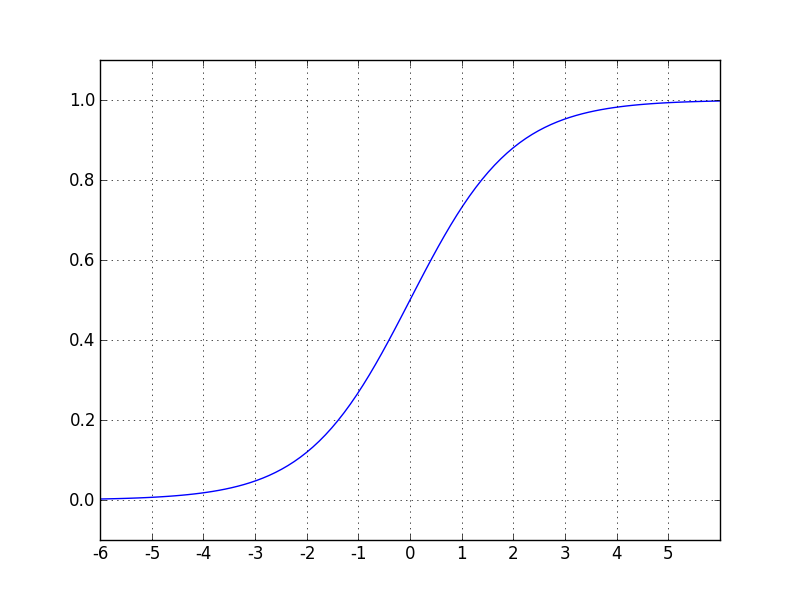
\includegraphics[width=0.8\linewidth,natwidth=898,natheight=587]{billeder/activationFunctions/sigmoid.png}
\caption{Sigmoid}
\label{fig:Sigmoid}
\end{figure}

\begin{figure}[H]
\centering
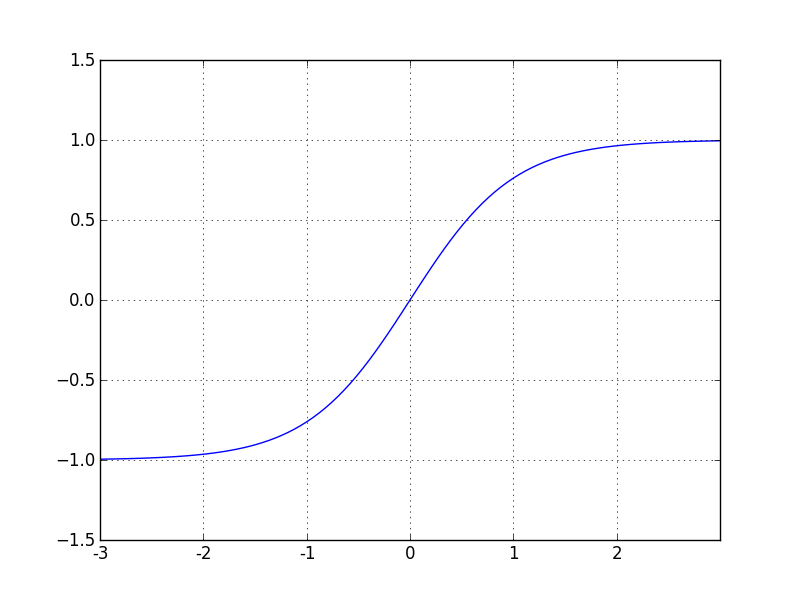
\includegraphics[width=0.8\linewidth,natwidth=898,natheight=587]{billeder/activationFunctions/tanh.png}
\caption{Hyperbolic tangent(tanh)}
\label{fig:Tanh}
\end{figure}

The normalization of the data is done using the following functions:
\begin{table}[H]
\centering  % used for centering table
\renewcommand{\arraystretch}{2}
\begin{tabular}{c c} % centered columns
 \#Normalization & \#Function \\ [0.5ex] % inserts table 
%heading
\hline                  % inserts single horizontal line
Zero-to-one & $ X_{norm} = \frac{X_i - X_{min}}{X_{max} - X_{min}}$ \\
Minus-one-to-one & $ X_{norm} = \frac{X_i - (\frac{X_{max} - X_{min}}{2})}{\frac{X_{max} - X_{min}}{2}}$ \\
[1ex]
\hline %inserts single line
\end{tabular}
\caption{Normalization functions} % title of Table
\label{table:naiveTrainingApproach} % is used to refer this table in the text
\end{table}
Where $X_i$ is the data entry, $X_min$ is the lowest value in the data set and $X_max$ is the highest value in the dataset.

\subsubsection{The naive approach}
First of all we tried out the most simple approach available, the naive approach, since this has almost no overhead and takes no preprocessing of the data. The method is simple; you take one neuron per input and one neuron as output. You add all of the data in your training set without doing any preprocessing of data. This kind of training set is good enough for simple problems e.g. the XOR problem or likewise. When we talk about more complex real-world problems like forecasting the energy prices this method does not perform to well and gives less than satisfactory results. Another factor is that a huge part of getting a neural network to perform well is the manipulation of the dataset to get rid of outliers and some of the noise in the dataset. Nevertheless it still gives an indication whether you have some kind of coherence between your input data and the output data even though the peromance is less than satisfactory.

\subsubsection{Trimming}
As mentioned before we need to get rid of some of the outliers and some of the noise in the data set to make it easier for the network to approximate a function based on the input data. There are different approaches to trimming but the two we use are standard trimming and percentile trimming of the dataset. Standard trimming is a simple way of getting rid of the worst outliers. The way to do it is; take a low and a high number in your data set and remove everything below and above these limits. Of course this can be very arbitrary but with a simple plot diagram you will be able to see where the limits should be set. Percentile trimming is a statistic approach where you cut of x\% from the top and the bottom of your dataset. You make a percentwise distribution over your dataset with the lowest values in the beginning and the highest values in the end. Then you can take the 5th percentile which represents the lowest 5\% of your dataset and the remove these values. The same is done for the top 5\% and then you have removed the most extreme outliers and made your dataset more robust in statistical analysis.
LAV GRAF DER VISER TRIMMING

\subsubsection{Matrix}
When analysing the data it is possible to find connection between different rows of data eg. what time of the day or what day of the week it is. These kind of data can be describe using a single node where you normalize the data between -1 and 1 but this will only give this neuron one weight to change for ALL the hours in the day. One approach to making these inputs more important than others are splitting them up into a simple matrix. This means that we have a matrix with one row and 24 inputs(one for each hour); we set a 1 in the input representing the time of day and set the rest to 0. This way the neural network will have a specific weight to apply according to which hour of the day it is. This of course adds alot of overhead in terms of how many input nodes you need to have and how many nodes you need in the hidden layers. This will increase the processing time of the neural network iterations so you have to do some cost/benefit analysis on it.

\subsubsection{Historical data}
Se step-ahead forecasting.

\subsubsection{Conclusion}
